\documentclass[journal,12pt,onecolumn]{IEEEtran}
\usepackage{cite}
 \usepackage{caption}
\usepackage{graphicx}
\usepackage{amsmath,amssymb,amsfonts,amsthm}
\usepackage{algorithmic}
\usepackage{graphicx}
\usepackage{textcomp}
\usepackage{xcolor}
\usepackage{txfonts}
\usepackage{listings}
\usepackage{enumitem}
\usepackage{mathtools}
\usepackage{gensymb}
\usepackage{comment}
\usepackage[breaklinks=true]{hyperref}
\usepackage{tkz-euclide} 
\usepackage{listings}
\usepackage{gvv}
%\def\inputGnumericTable{}                                 
\usepackage[latin1]{inputenc} 
\usetikzlibrary{arrows.meta, positioning}
\usepackage{xparse}
\usepackage{color}                                            
\usepackage{array}                                            
\usepackage{longtable}                                       
\usepackage{calc}                                             
\usepackage{multirow}
\usepackage{multicol}
\usepackage{hhline}                                           
\usepackage{ifthen}                                           
\usepackage{lscape}
\usepackage{tabularx}
\usepackage{array}
\usepackage{float}

\usepackage{float}
%\newcommand{\define}{\stackrel{\triangle}{=}}
\theoremstyle{remark}
\usepackage{circuitikz}
\captionsetup{justification=centering}
\usepackage{tikz}

\title{Matrices in Geometry 8.4.38}
\author{EE25BTECH11035 - Kushal B N}
\begin{document}
\vspace{3cm}
\maketitle
{\let\newpage\relax\maketitle}
\textbf{Question: }
Let $0 < \theta < \frac{\pi}{2}$. If the eccentricity of the hyperbola $\frac{x^2}{\cos^2{\theta}} - \frac{y^2}{\sin^2{\theta}} = 1$ is greater than 2, then the length of its latus rectum lies in the interval
\begin{enumerate}
    \item $(5,\infty)$
    \item $(\frac{3}{2},3 ]$
    \item $(2,3]$
    \item $(1,\frac{3}{2}]$
\end{enumerate}

\textbf{Given: }

Hyperbola $\sec^2(\theta)x^2 - \csc^2(\theta)y^2 = 1$ for which $e>2$

\textbf{Solution: }\\

Comparing to the general conic form $\vec{x}^{\top}\vec{V}\vec{x} + 2\vec{u}^{\top}\vec{x} + f = 0$, we get

\begin{equation}
    \vec{V} = \myvec{\sec^2(\theta) & 0\\0 & \csc^2(\theta)}
\end{equation}

\begin{equation}
    \vec{u} = \myvec{0\\0}
\end{equation}

\begin{equation}
    f = -1
\end{equation}

Now, here as $\vec{V}$ is a diagonal matrix, its eigenvalues are its diagonal entries, that is,
\begin{equation}
    \lambda_1 = \frac{1}{\sin^2{\theta}}
\end{equation}
\begin{equation}
    \lambda_2 = \frac{1}{\cos^2{\theta}}
\end{equation}

Now, the eccentricity of the hyperbola
\begin{equation}
    e = \sqrt{1 - \frac{\lambda_1}{\lambda_2}}
\end{equation}

\begin{equation}
    \implies e^2 = 1 + \frac{\sin^2{\theta}}{\cos^2{\theta}} = \frac{1}{\cos^2{\theta}}
\end{equation}

As $0 < \theta < \frac{\pi}{2}$, $\cos{\theta}$ is positive and so,
\begin{equation}
    e = \frac{1}{\cos{\theta}}
\end{equation}

Now, as $e > 2$
\begin{equation}
    \frac{1}{\cos{\theta}} > 2 \implies \cos{\theta} < \frac{1}{2}
\end{equation}

\begin{equation}
    \implies \frac{\pi}{3} < \theta < \frac{\pi}{2}
    \label{eq10}
\end{equation}

Length of the latus rectum,
\begin{equation}
    l = \frac{2\sqrt{\abs{f_0\lambda_1}}}{\abs{\lambda_2}}
    \label{eq11}
\end{equation}

where,
\begin{equation}
    f_0 = \vec{u}^{\top}\vec{V}^{-1}\vec{u} - f
\end{equation}

as $\vec{u} = \myvec{0\\0}$, we get
\begin{equation}
    f_0 = -f = -(-1) = 1
\end{equation}

Substituting these values into \eqref{eq11}, we get
\begin{equation}
    l = \frac{2\sqrt{\abs{1.\sec^2\theta}}}{\abs{\csc^2\theta}}
\end{equation}

In the interval $0 < \theta < \frac{\pi}{2}$, $\sec\theta$ is positive and so
\begin{equation}
    \implies l = \frac{2\sin^2{\theta}}{\cos{\theta}}
\end{equation}

Now from \eqref{eq10}, we get
\begin{equation}
    \fbox{$l \in (3,\infty)$}
\end{equation}

\textbf{Final Answer: }

The length of the latus rectum for the given hyperbola lies in the interval $(3,\infty)$.

\begin{figure}[H]
    \centering
    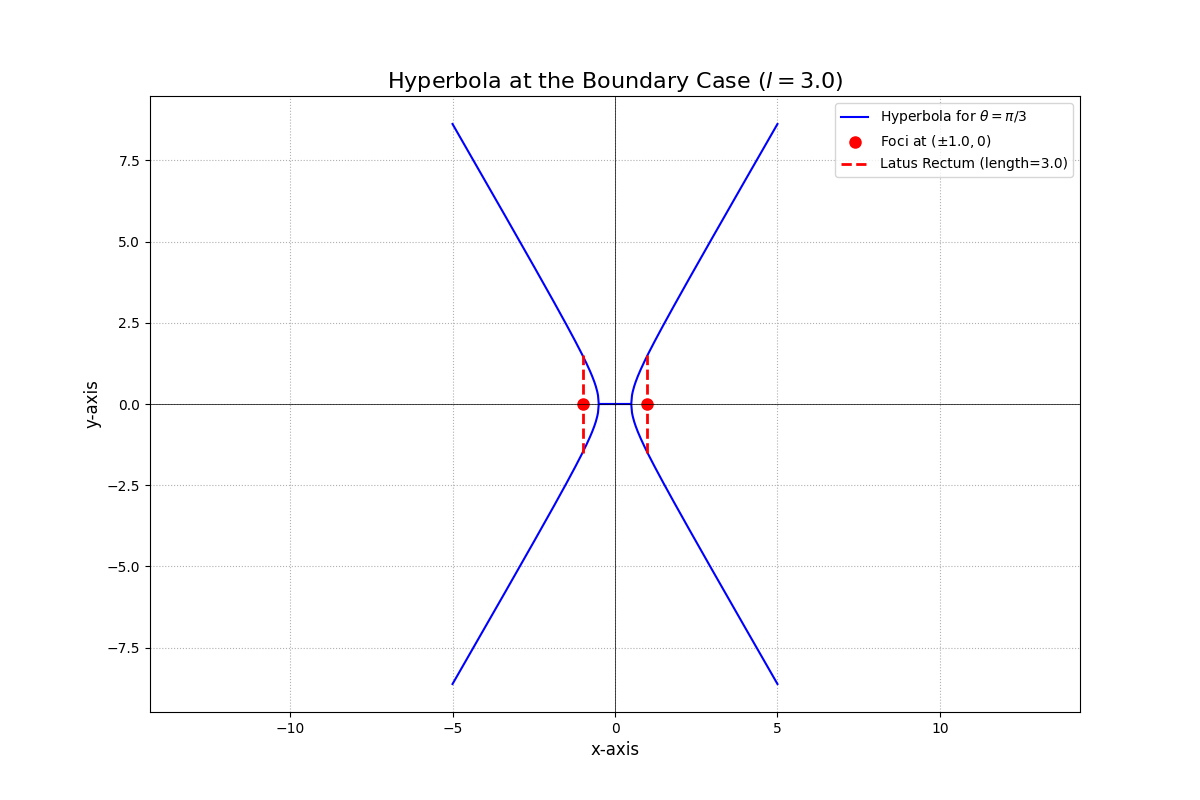
\includegraphics[width=0.75\columnwidth]{figs/1.png}
    \caption{Plot for 8.4.38}
\end{figure}
\end{document}
